\section{Interference Bound Function}
In the worst case release pattern, we can easily calculate the exact value of $dbf(\tau_i,t)$. However the exact value of $ibf_i(\tau-\tau_i,t')$ is not trivial except we simulate the system.  As a result, here we need to add some pessimism to bound the actual value of  $ibf_i(\tau_j,t')$ instead. We will also apply an optimization technique to further improve the performance of the test because the resource consumed by $\tau$ before $r_{i,x}$ or $P_{i,x}$ can not be greater than $r_{i,x}$ or $P_{i,x}$, respectively. Thus here we also derive  $ibf_i^1(\tau_j,t')$ and $ibf_i^2(\tau_j,t')$ which denote the maximum possible resource consumed by  $\tau_j$ after $r_{i,x}$ and $P_{i,x}$, respectively.  



In the worst case pattern, given a time interval length $t$, we can easily calculate the release time and promotion point of each job.
Here we first present some notations that  will be used later in the paper.
\begin{table}[h]
\caption{Notations}
\label{tab:x}
\center
\begin{tabular}{|l|l|l|l|}
 \hline
 $P_{i,x}=t-D_i+p_i$ & $r_{i,x}=P_{i,x}-p_i$ & $n_j=\lfloor \frac{t'}{T_j}\rfloor$ \\
 \hline
 $r_{j,y}=n_j\times T_j$ &$P_{j,y}=r_{j,y}+p_j$ &$[a]_0=\max(a,0)$\\
 \hline
$n_j'=\lfloor \frac{r_i}{T_j}\rfloor$  & $r_{j,y'}=n_j'\times T_j$& $[a,b]_s=\min(a,b)$\\
 \hline
	$n_j''=\lfloor \frac{P_{i,x}}{T_j}\rfloor$ &  $r_{j,y''}=n_j''\times T_j$&	 $[a,b]_g=\max(a,b)$\\
  \hline
\end{tabular}
\end{table}


Suppose $J_{j,y}$ is the job that has its release time $r_{i,x}\leq t'\leq r_{i,x}+T_j$, then we only need to figure out how much resource  $J_{j,y}$ has consumed by $t'$.  This is because that the $n_j$ previous jobs released before  $r_{j,y}$ are assumed to meet their deadlines, and hence are supposed to consume $n_j.C_j$ time units of resource. 

\subsection{$ibf_i(\tau_j,t')$ when $j<i$}
We first consider the case when index $j$ is smaller than index $i$ which means $\tau_j$ has higher origin priority than $\tau_i$. Thus if  $J_{j,y}$ is still active, $J_{i,x}$ would not  execute unless it is during the interval $[P_{i,x}, P_{j,y}]$ (if $P_{i,x}<P_{j,y}$).


\textbf{Case 1 ( $P_{j,y}\leq P_{i,x}$)} as shown in  Figure~\ref{fig:case1}: Job $J_{i,x}$ always has lower priority than  $J_{j,y}$. Thus   the maximum possible resource consumed by $\tau_{j}$  before $t'$ is  bounded by
	\begin{align*}
		ibf_i(\tau_j,t')=n_j.C_j +\min\left(C_j,t'-r_{j,y}\right)
	\end{align*}
 

\begin{figure}[h!]
 \centering
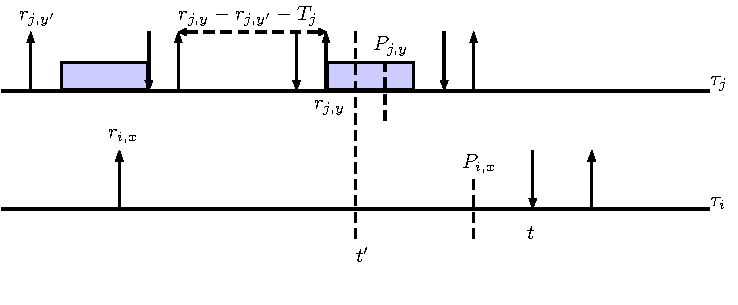
\includegraphics[scale=0.7]{Figure/C1}  
\caption{$ P_{j,y}\leq P_{i,x}$}
  \label{fig:case1}
\end{figure}

The resource $\tau_j$ consumes  after $r_{i,x}$ or $P_{i,x}$ is maximized when its execution happens as late as possible as shown in Figure~\ref{fig:case1}, and hence we have
	\begin{align*}
	\begin{split}
	ibf_{i}^1(\tau_j,t')=~~~~~~~~~~~~~~~~~~~~~~~~~~~~~~~~~~~~~~~~\\
	\begin{cases}
	&\min(C_j, t'-r_{i,x})~\mbox{~~~~~~~~~~if } r_{j,y}\leq r_{i,x}\\
	&\min(C_j, t'-r_{j,y})+\min(C_j,[r_{j,y'}+D_j-r_{i,x}]_0)\\
	&+\frac{r_{j,y}-r_{j,y'}-T_j}{T_j}C_j \mbox{~~~~~~~~~~~~~if~} r_{j,y}>r_{i,x}\\
	\end{cases}
	\end{split}
	\end{align*}
Its maximum possible execution after $P_{i,x}$ is
	\begin{align*}
	\begin{split}
	ibf_{i}^2(\tau_j,t')=~~~~~~~~~~~~~~~~~~~~~~~~~~~~~~~~~~~~~~\\
	\begin{cases}
	&\min\{C_j, [t'-P_{i,x}]_0\}\mbox{~~~~~~~~~~~~~if } r_{j,y}\leq P_{i,x}\\
	&\min\{C_j, t'-r_{j,y}\}+\frac{r_{j,y}-r_{j,y''}-T_j}{T_j}C_j+\\&\min(C_j,[r_{j,y''}+D_j-P_{i,x}]_0)  \mbox{~~~~if } r_{j,y}>P_{i,x}
	\end{cases}
	\end{split}
	\end{align*}





\begin{figure}[h!]
 \centering
\includegraphics[scale=0.7]{Figure/C2}  
\caption{$P_{j,y}> P_{i,x}$}
  \label{fig:case2}
\end{figure}

\textbf{Case 2} ($P_{j,y}> P_{i,x}$):~as shown in  Figure~\ref{fig:case2}, $J_{i,x}$ has higher priority than $J_{j,y}$'s  during $[\max(r_{j,y},P_{i,x}),P_j]$ (if $P_i\leq P_j$). Thus  $J_{j,y}$ can not execute  during $[\max(r_{j,y},P_{i,x}),P_j]$ unless $J_{i,x}$ has already finished. Thus we have
	\begin{align*}
		&ibf_i(\tau_j,t')=n_j.C_j +
\\&\min\left(C_j,\!t'\!-\!r_{j,y}\!-\!\left(\min(t'\!,\!P_{j,y})\!-\!\max(r_{j,y},\!P_{i,x})\right)\right)
		\end{align*}

Its maximum possible execution after $r_{i,x}$ is
\begin{align*}
\begin{split}
ibf_{i}^1(\tau_j,t')=~~~~~~~~~~~~~~~~~~~~~~~~~~~~~~~~~~~~~~~~~~~~~~\\
\begin{cases}
&\min(C_j,\min(t',P_{i,x})-r_{i,x})\\&\mbox{~~~~~~~~~~~~~~~~~~~~~~~~~~~~if } t'<P_{j,y}\wedge r_{j,y}\leq r_{i,x}\\
&\min(C_j,\min(t',\max(r_{j,y},P_{i,x}))-r_{j,y})+\\&\frac{r_{j,y}-r_{j,y'}-T_j}{T_j}C_j +\min(C_j,[r_{j,y'}+D_j-r_i]_0)\\
&\mbox{~~~~~~~~~~~~~~~~~~~~~~~~~~~~if } t'<P_{j,y}\wedge r_{j,y}> r_{i,x}\\
&\min\{C_j,t'-r_{i,x}-(P_{j,y}-P_{i,x})\}\\
&\mbox{~~~~~~~~~~~~~~~~~~~~~~~~~~~~if } t'\geq P_{j,y}\wedge r_{j,y}\leq r_{i,x}\\
&\min\{C_j,t'-r_{j,y}-(P_{j,y}-\max(r_{j,y},P_{i,x}))\}\\ &+\frac{r_{j,y}-r_{j,y'}-T_j}{T_j}C_j+\min(C_j,[r_{j,y'}+D_j-r_{i,x}]_0)\\
&\mbox{~~~~~~~~~~~~~~~~~~~~~~~~~~~~if } t'\geq P_{j,y}\wedge r_{j,y}> r_{i,x}\\
\end{cases}
\end{split}
\end{align*}
Its maximum possible execution after $P_{i,x}$ is
\begin{align*}
\begin{split}
ibf_{i}^2(\tau_j,t')=~~~~~~~~~~~~~~~~~~~~~~~~~~~~~~~~~~~~~~~~~~\\
\begin{cases}
&0\mbox{~~~~~~~~~~~~~~~~~~~~~~~~~~~if } t'<P_{j,y} \wedge r_{j,y}\leq P_{i,x}\\
&\frac{r_{j,y}-r_{j,y''}-T_j}{T_j}C_j+\min(C_j,[r_{j,y''}+D_j-P_{i,x}]_0)\\&
\mbox{~~~~~~~~~~~~~~~~~~~~~~~~~~~~if } t'<P_{j,y} \wedge r_{j,y}> P_{i,x}\\
&\min\{t'-P_{j,y},C_j\}\mbox{~~~~~~~if } t'\geq P_{j,y} \wedge  r_{j,y}\leq P_{i,x}\\
&\min\{t'-P_{j,y},C_j\}+\min(C_j,[r_{j,y''}+D_j-P_{i,x}]_0)\\
&+\frac{r_{j,y}-r_{j,y''}-T_j}{T_j}C_j\mbox{~~~~~~~~~~if } t'\geq P_{j,y} \wedge  r_{j,y}> P_{i,x}\\
\end{cases}
\end{split}
\end{align*}


% % %



% 
\subsection{$ibf_i(\tau_j,t')$ when $j> i$}
 
\textbf{Case 1.1} ($P_{i,x}\leq P_{j,y}\wedge r_{j,y}\leq r_{i,x}$): as shown in  Figure~\ref{fig:case3}, $\tau_j$ may execute during $[r_{j,y},r_{i,x}]$, but $\tau_j$ would not execute after $r_{i,x}$  unless $\tau_i$ has finished.

	\begin{figure}[h!]
 \centering
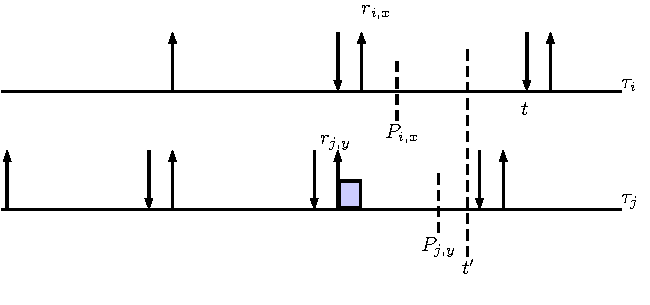
\includegraphics[scale=0.7]{Figure/C3}  
\caption{$P_i\leq P_j\wedge r_j\leq r_i$}
  \label{fig:case3}
\end{figure}
		\begin{align*}
		ibf_i(\tau_j,t')=n_j\times C_j+\min(C_j,r_{i,x}-r_{j,y})
	\end{align*}
However $J_{j,y}$ would never execute after $r_{i,x}$, and hence we have
\begin{align*}
&ibf_{i}^1(\tau_j,t')=\min(C_j,r_{i,x}-r_{j,y})
\end{align*}


\begin{align*}
\begin{split}
ibf_{i}^2(\tau_j,t')=0
\end{split}
\end{align*}


\textbf{Case 1.2} ($P_{i,x}\leq P_{j,y}\wedge r_{j,y}> r_{i,x}$): as shown in  Figure~\ref{fig:case4},  $J_{j,y}$ would not execute unless $\tau_i$ has completed. Thus we have
\begin{align*}
		ibf_i(\tau_j,t')=n_j\times C_j
\end{align*}

\begin{figure}[h!]
 \centering
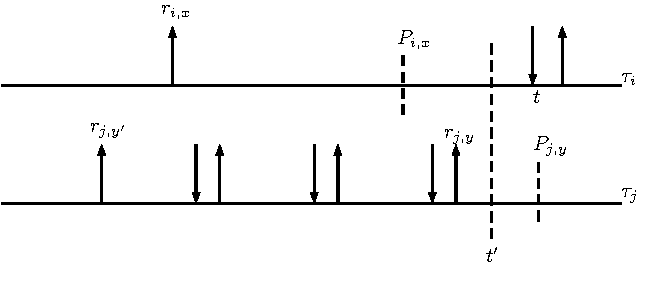
\includegraphics[scale=0.7]{Figure/C31}  
\caption{$P_{i,x}\leq P_{j,y}\wedge r_{j,y}> r_{i,x}$}
  \label{fig:case4}
\end{figure}
$\tau_j$ would not execute $P_{i,x}$ unless $J_{i,x}$ has already finished. Therefore we have
\begin{align*}
ibf_{i}^2(\tau_j,t')=0
\end{align*}

 To maximize the possible execution of $\tau_j$ after $r_{i,x}$, we assume $\tau_j$ executes as late as possible. Meanwhile   $J_{j,y-1}$  can not execute after $r_{j,y-1}+D_j$ or $P_{i,x}$ (if $P_{j,y-1}<P_{i,x}$) unless $J_{i,x}$ completes.


\begin{align*}
&ibf_{i}^1(\tau_j,t')=\\
&\frac{r_{j,y}-r_{j,y'}-T_j}{T_j}C_j+\min(C_j,[r_{j,y'}+D_j-r_{i,x}]_0)
\end{align*}

% % \my{


\textbf{Case 2.1} ($P_{i,x}>P_{j,y}\wedge r_{j,y}\leq r_{i,x}$): as shown in  Figure~\ref{fig:case5}, the last job of $\tau_j$ can execute until $\min(t',P_i)$
	\begin{align*}
		&ibf_i(\tau_j,t')=n_j\times C_j+\\
		&\min\left(C_j,r_{i,x}-r_{j,y}+[\min(t',P_{i,x})-\max(P_{j,y},r_{i,x})]_0\right)
	\end{align*}
	\begin{align*}
ibf_{i}^1(\tau_j,t')=\min\{C_j,[\min(t',P_{i,x})-\max(P_{j,y},r_{i,x})]_0\}
\end{align*}
\begin{align*}
\begin{split}
rbf_{i}^2(\tau_j,t')=0
\end{split}
\end{align*}

\begin{figure}[h!]
 \centering
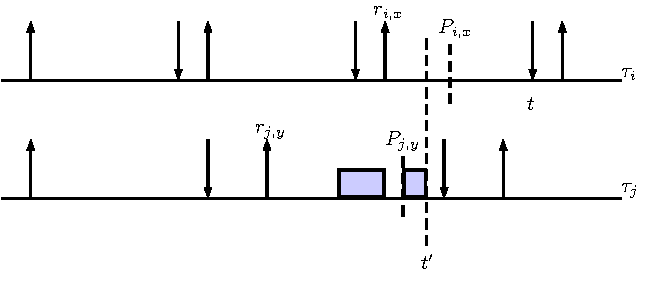
\includegraphics[scale=0.7]{Figure/C4}  
\caption{$P_{i,x}>P_{j,y}\wedge r_{j,y}\leq r_{i,x}$}
  \label{fig:case5}
\end{figure}

\begin{figure}[h!]
 \centering
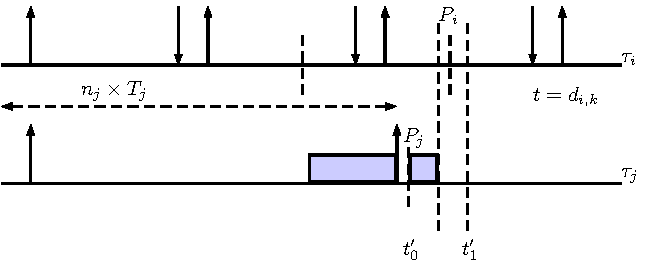
\includegraphics[scale=0.7]{Figure/C41}  
\caption{$P_{i,x}>P_{j,y}\wedge r_{j,y}> r_{i,x} $}
  \label{fig:case6}
\end{figure}

\textbf{Case 2.2} ($P_{i,x}>P_{j,y}\wedge r_{j,y}> r_{i,x}$): as shown in  Figure~\ref{fig:case6}, $J_{j,y}$ would only execute during $[P_{j,y},P_{i,x}]$ before $J_{i,x}$ finishes. Thus we have
\begin{align*}
	ibf_i(\tau_j,t')=n_j.C_j+\min\left(C_j,[\min(t',P_{i,x})-P_{j,y}]_0\right)
\end{align*}


\begin{align*}
&ibf_{i}^1(\tau_j,t')=\min(C_j,[r_{j,y'}+D_j-r_{i,x}]_0)+\\
&\min\left(C_j,[\min(t',P_{i,x})-P_{j,y}]_0\right)+\frac{r_{j,y}-r_{j,y'}-T_j}{T_j}C_j
\end{align*}

\begin{align*}
rbf_{i}^2(\tau_j,t')=0
\end{align*}





\section{Optimization Technique}
We can bound the total execution before $r_i$ or $P_i$ (if $t'>P_i$) by $r_i$ or $P_i$, respectively. For $\tau_i$ itself, we simply assume its execution demand after $r_i$ and $P_i$ is $C_j$.

\begin{equation}
F_1(\tau_i,t,t')=\min\left(r_i,n_i\times C_i+\sum_{\tau_j\in\{\tau-\tau_i\}}rbf_i(\tau_j,t')-rbf_{i}^1(\tau_j,t')\right)+\sum_{\tau_j\in\{\tau-\tau_i\}}rbf_{i}^1(\tau_j,t')+C_i
\end{equation}


\begin{equation}
F_2(\tau_i,t,t')=\min\left(P_i,n_i\times C_i+\sum_{\tau_j\in\{\tau-\tau_i\}}rbf_i(\tau_j,t')-rbf_{i}^2(\tau_j,t')\right)+\sum_{\tau_j\in\{\tau-\tau_i\}}rbf_{i}^2(\tau_j,t')+C_i
\end{equation}

\begin{equation}
\begin{split}
F(\tau_i,t,t')=
\begin{cases}
F_1(\tau_i,t,t')&\mbox{if } t'<=P_i\\
\min\{F_1(\tau_i,t,t'),F_2(\tau_i,t,t')\}&\mbox{otherwise}
	\end{cases}	
\end{split}
\end{equation}




We can derive a simple upper bound of $t$. Suppose that
\[
\forall~t'\in(k.T_i,k.T_i+D_i]:~F(\tau_i,t,t')>t'\Rightarrow\min_{t'\in(k.T_i,k.T_i+D_i]}\frac{F(\tau_i,t,t')}{t'}>1
\]
, and let
\[
H_i(t)=  U\times t+\sum_{\tau_j\in\{\tau-\tau_i\}}C_j\geq t\times u_i+(\lfloor \frac{t'}{T_j} \rfloor+1)C_j\geq F(\tau_i,t,t')
\]

then it must be that

\begin{align*}
\frac{H_i(t)}{t-D_i}>1\Rightarrow t-D_i< U\times t+\sum_{\tau_j\in\{\tau-\tau_i\}}C_j\Rightarrow t<\frac{D_i+\sum_{\tau_j\in\{\tau-\tau_i\}}C_j}{1-U}
\end{align*}

% \section{Draft Simulation Results}

% \begin{table}[h]
% \caption{Notations}
% \label{tab:x}
% \large
% \center
% \begin{tabular}{|l|l|l|l|l|}
%  \hline
% Uniform Distribution&[0.88,0.9]&[0.93,0.95]&[0.95,0.97]&[0.97,0.99]\\
%  \hline
% Acceptance Ratio&1&1&0.995&0.982\\
%  \hline
% \end{tabular}
% \end{table}